\documentclass{article}
\usepackage[utf8]{inputenc}
\usepackage{hyperref}

\author{Meng Lu, Paula Moraga }
\date{September 2020}
\usepackage{amsmath}
\usepackage{natbib}
\usepackage{graphicx}
\usepackage{listings} 
\lstset{language=R,
    breaklines=true,
    basicstyle=\small\ttfamily,
    stringstyle=\color{DarkGreen},
    otherkeywords={0,1,2,3,4,5,6,7,8,9},
    morekeywords={TRUE,FALSE},
    deletekeywords={data,frame,length,as,character}
}
\usepackage{cleveref}


\title{A comparison of INLA and machine learning-based methods in $NO_2$ modelling: prediction accuracy, uncertainty quantification, and interpretability }
\begin{document}

\maketitle
\begin{abstract} 
Machine learning methods have been applied in NO$_2$ mapping and in several model comparison studies compared between each other and to data model-based methods including linear regression and Kriging. However, current studies rarely compare and discuss uncertainty quantification and interpretability across these methods. In this study, we focus on distribution prediction methods developed in INLA and Random Forest and the interpretability of the models, the findings are extensible to boosting ensemble-tree methods. Further, we compare a linear INLA, Lasso, Random Forest, and XGboost, and evaluated stack learning methods, with and without modeling spatial variations, in mapping NO$_2$ at European country level. We used national ground station measurements of NO$_2$ in Germany and Netherlands, of the year 2017, and the NO$_2$ prediction grid is at 100 m by 100 m resolution.   
\end{abstract}

\section{Introduction}
Ensemble tree-based Machine learning (ML) methods (e.g. random forest, boosting) have been introduced in statistical air pollution modelling and have been compared in \cite{chen2019comparison,kerckhoffs2019performance,luglobal}. However, in all the studies, comparisons are only based on the cross-validation accuracy of prediction mean, ignoring the prediction distributions for uncertainty quantification. Also not discussed is the ability and limitation of the ML methods in modeling the spatial effects and informing error sources (e.g. if the errors are due to missing co-variates or model structure). Consequently, current model comparison studies maybe one-sided. In this study, our objectives are to:
\begin{enumerate}
    \item Compare ML and Gaussian process models for the reliability of their distribution and mean predictions, and their potential in providing information for model improvement (indicating missing co-variates).
    
    \item Propose an optimal statistical model that models the spatial random effects in stacked learning.
\end{enumerate}

The first goal is achieved by comparing INLA with three ML methods: Lasso, XGBoost, and Random Forest (RF). The four methods are chosen for their dissimilarity: Lasso is a linear model without accounting for spatial dependency, which is modelled in INLA as spatial random effects. RF and XGBoost are non-linear and are not affected by dependent co-variates, with the later build tree models subsequently over the residuals of previous trees and has multiple routines to penalise model over-fittng, which has been reported in various studies to obtain the highest prediction accuracy. Among the ML methods, only the distribution prediction and interpretability from INLA and RF are compared, as INLA is representative to Gaussian process models and RF an ensemble tree model.

The second goal is achieved by using a Gaussian process to stack machine learners as a super-learner (cite), to compare the modelled spatial random effects with the super-learner that does not model the spatial random effects. 

 
 
\section{Data}
We used average NO2 concentration of 2017 from ground stations in Netherlands and Germany.

\subsection{Variables used in INLA modeling} 
The INLA is used in two models:  applying to predictor variables as other methods and stacked modeling. Before applying INLA to predictor variables, we used Lasso to reduce the number of variables. The Lasso is used in contrast to ensemble tree-based methods as they are both linear models. We bootstrapped data 20 times, and used the variables that are selected more than 10 times to consider. The frequency that the Lasso selected a certain variable is shown in \cref{lassoselect}.

  \begin{table}[!htbp] \centering 
  \caption{Variables selected by Lasso, frequency indicates the number of times the variables are selected in 20 times boot-strapping. (we can only select variables that appear more than 5 times to consider).} 
  \label{lassoselect} 
\begin{tabular}{@{\extracolsep{5pt}} ccc} 
\\[-1.8ex]\hline 
\hline \\[-1.8ex] 
 & Variables & Frequency \\ 
\hline \\[-1.8ex] 
 1 & nightlight\_450 & $20$ \\ 
2 & population\_1000 & $20$ \\ 
3 & population\_3000 & $20$ \\ 
4 & road\_class\_1\_5000 & $20$ \\ 
5 & road\_class\_2\_100 & $20$ \\ 
6 & road\_class\_3\_300 & $20$ \\ 
7 & trop\_mean\_filt & $20$ \\ 
8 & road\_class\_3\_3000 & $19$ \\ 
9 & road\_class\_1\_100 & $18$ \\ 
10 & road\_class\_3\_100 & $14$ \\ 
11 & road\_class\_3\_5000 & $6$ \\ 
12 & road\_class\_1\_300 & $5$ \\ 
13 & road\_class\_1\_500 & $5$ \\ 
14 & road\_class\_2\_1000 & $2$ \\ 
15 & nightlight\_3150 & $1$ \\ 
16 & road\_class\_2\_300 & $1$ \\ 
17 & road\_class\_3\_1000 & $1$ \\ 
18 & temperature\_2m\_7 & $1$ \\  
 
\hline \\[-1.8ex] 
\end{tabular} 
\end{table} 

\section {method}

\subsection{Models}
\subsubsection{INLA}
%PAULA
\subsubsection{Machine learning methods}

\subsubsection{Stacked learning}
Stacked learning is trained based on the cross-validation of different learners, in this case the three learners are random forest, XGBoost, and Lasso. Two super learners are compared, one is the native optimisation, and the other using the gaussian process to also model the spatial random effects. 

\subsection {Prediction intervals}
Prediction quantiles and coverage probability are calculated for each method for uncertainty quantification. The coverage probability is calculated as the ratio between the number of  predictions within the upper and lower quantile and the total number of predictions. The prediction quantiles for each methods are calculated as following:
\begin{itemize}
     
\item INLA
%PAULA

\item Random Forest 
 The predictive quantiles of RF are calculated in two ways, one is uses all the observations in each terminal node and over all the trees as a predicted distribution for each terminal node, known as quantile regression forest \citep{meinshausen2006quantile}. The second method embeds the GAMLSS \citep{stasinopoulos2007generalized} into random forest, known as distributional forests \citep{schlosser2019distributional}, which for each tree uses standard maximum likelihood to fit distributions and recursively select and split co-variates according to the instability of the gradient of the likelihood at each observation along each co-variate. For interpretability, we compared the impact of a certain co-variate on model predictions, by analysing the coefficients estimated by INLA and Lasso and the tree SHAP \citep[SHapley Additive exPlanations,][]{lundberg2018explainable} estimated by RF and XGBoost.  

\subsection{Spatial validation}
Besides 20-times random bootstrapping, We also used four other spatial validation methods to comprehensively evaluate the models at different angles.

\begin{enumerate}
    \item Probability sampling: higher probability is given in selecting observations that are isolated, to test how good the model is at predicting air pollution over the whole region. This is because with random sampling we would get more points in areas where observations are clustered and may not pick any observation in areas with few observations.   
    \item Spatial blocked cv: divide the data into spatial blocks, each time use one block for validation and other blocks for predicting. 
    \item Validation based on customised predictors: based on predictor values, we divided the study area so that we assess the prediction accuracy for certain areas. In this study, three subareas are defined:  1) close to traffic and high population:  
    2) close to traffic and middle low population. 3) far away from traffic. High population is defined as the variable population of 1000 m buffer that is in the last quartile. Low population is defined as the variable population of 1000 m buffer is below the median. Close to road is defined as: 
    \begin{lstlisting} 
    
    road_class_2_100 > 0 | 
    road_class_1_100 > 0 |
    road_class_3_100 > quantile(road_class_3_100, .75)) \end{lstlisting}
    Far away from road is defined as:
  \begin{lstlisting} 
    road_class_2_100 == 0 &
    road_class_1_100 == 0 & 
    road_class_3_100 < quantile(road\_class\_3\_100, .5)
    
    \end{lstlisting}
    where "{\tt \&}" indicates "and" and "{\tt |}" indicates "or". the second variable of the function "{\tt quantile(.)}" indicates the percentage quantile of the variables. 
   
    \item Validation based on known attribute: we know the air quality station types (traffic, background, industrial) and human settlement types (urban or rural), this allows us to quantify prediction accuracy for each type of air quality stations and separating between urban and rural areas. 
\end{enumerate}

%\item XGboost
%Quantile regression is used to calculate the prediction quantiles of XGBoost, based on \cite{quantile} 

%\item Lasso

\end{itemize}
 
\section{Results}
\subsection{Prediction Accuracy}
\begin{table}[!htbp] \centering 
  \caption{Cross-validation results of 20 times boot-strapping.} 
  \label{cv} 
\begin{tabular}{@{\extracolsep{5pt}} ccccccc} 
\\[-1.8ex]\hline 
\hline \\[-1.8ex] 
   &LA & RF& XGB & stacked& INLA& stacked INLA  \\ 
\hline \\[-1.8ex] 	
 
RMSE & $7.8$ & $7.5$ & $7.4$ & 7.2 & 7.5&7.1\\
%RRMSE & $0.3$ & $0.3$ & $0.3$&  &0.3\\
%IQR & $8.5$ & $7.5$ & $6.9$  &  &7.2\\ % for non-gaussian error this makes little sense
%rIQR & $0.4$ & $0.3$ & $0.3$ & &0.3\\
MAE & $5.9$ & $5.5$ & $5.3$  & 5.2 & 5.5&5.3\\
%rMAE & $0.2$ & $0.2$ & $0.2$ &  &0.2\\
R$^2$ & $0.63$ & $0.66$ & $0.67$&  0.68 &0.66 &0.69\\
%explained\_var & $0.63$ & $0.66$ & $0.67$ &&  0.66 &0.69 \\ 
\hline \\[-1.8ex] 
\end{tabular} 
\end{table} 


\subsection{Distributional forest vs. quantile regression trees}

Both the distributional forest and quantile regression trees reach the coverage probability higher than 0.9, but the distributional forest predict a more realistic prediction quantile, notably, it covers four observations that are not covered by the prediction quantile predicted by the quantile regression forest. 

\begin{figure}
\centering
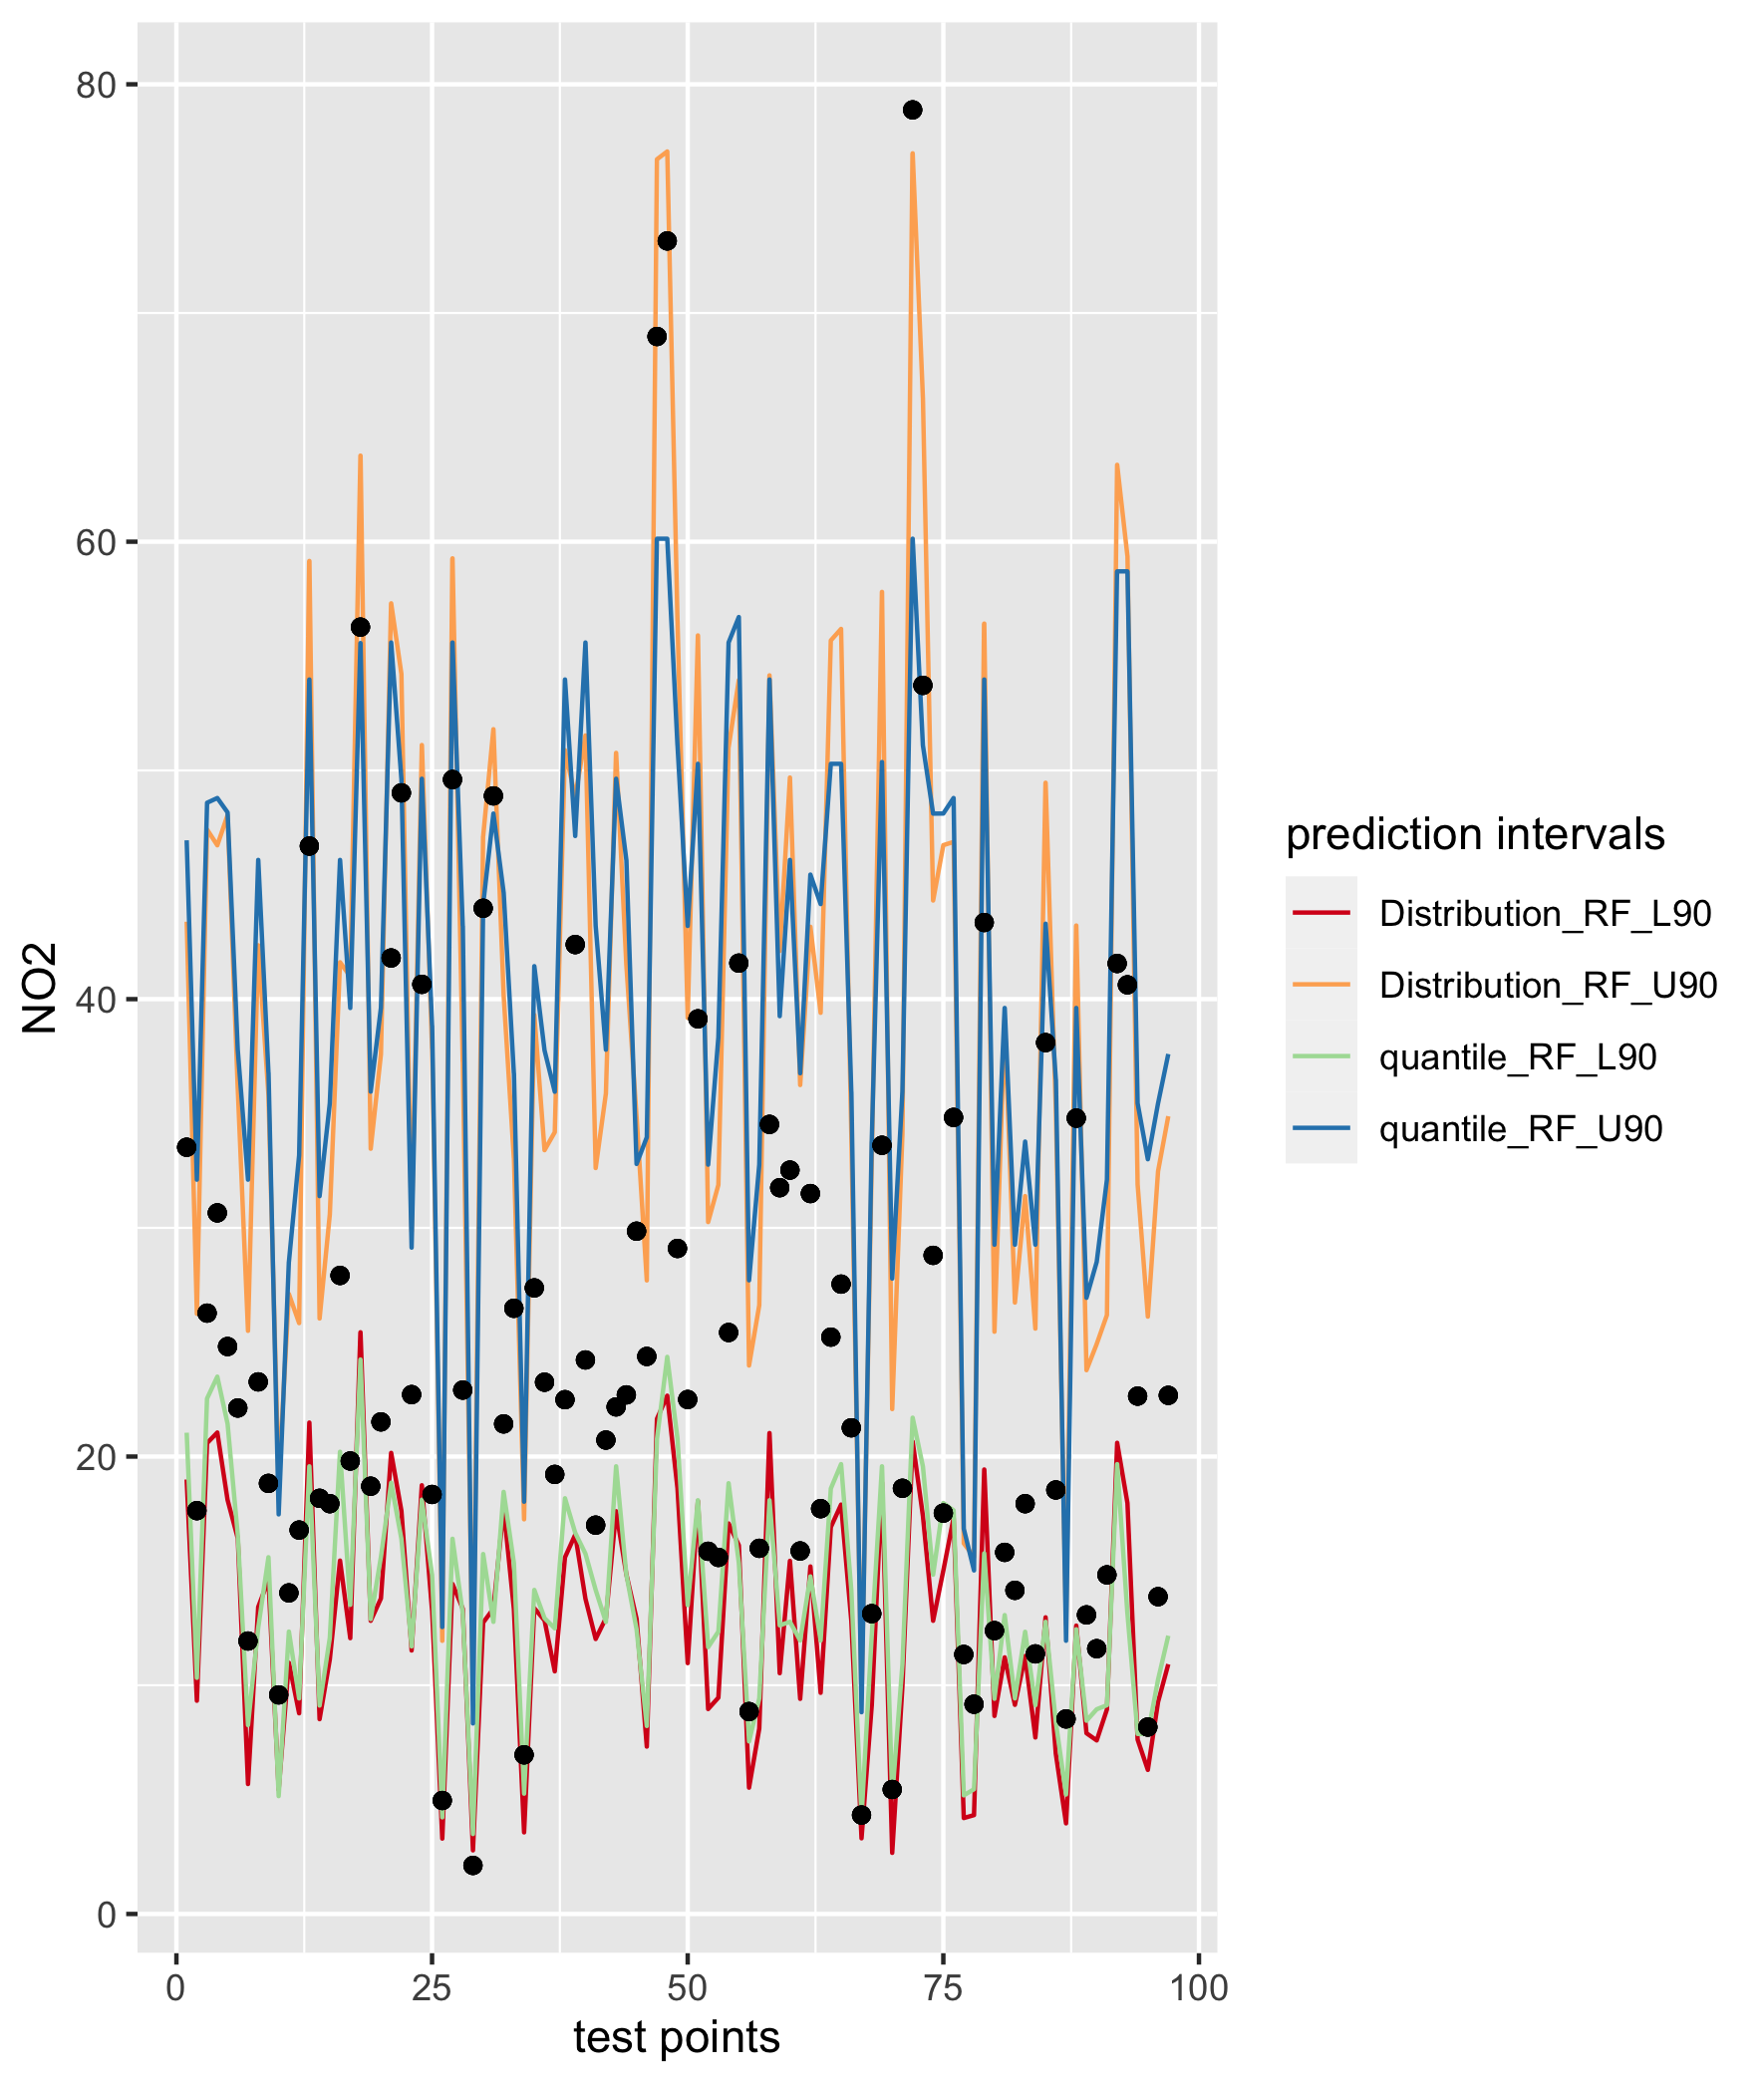
\includegraphics[scale = 0.2]{fig/dist_vs_qrf.png}
\caption{The 90\% prediction interval predicted by distributional forest and quantile regression trees. The black dots indicate observations in the test dataset.}
\label{distvsquant}
\end{figure}

\subsection{Interpretability} 
The INLA coefficients

SHAP variable impact for the RF and XGBoost, the variables are ranked by their variable importance. It can be observed from \cref{rfshap} and \cref{xgbshap} that the variable rankings differ but the number of points that have positive or negative impact are similar.  
% do they give the same interpretation?
\begin{figure}
\centering
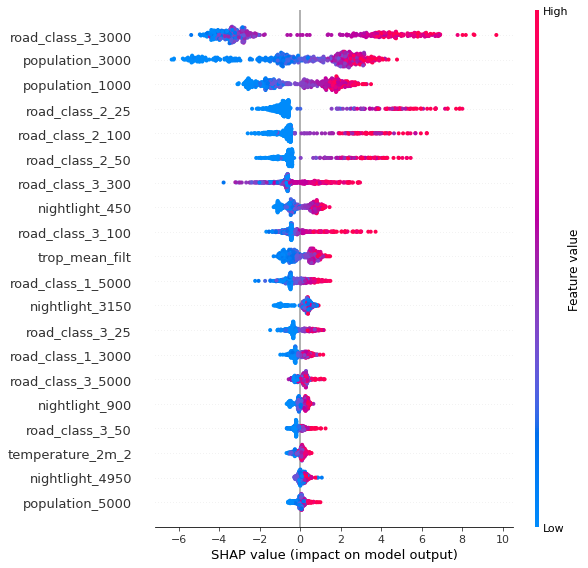
\includegraphics[scale = 0.5]{fig/rfshap.png}
\caption{Variable impact calculated by SHAP, the RF model. The horizontal location shows whether the effect of that value is associated with a higher or lower prediction.}
\label{rfshap}
\end{figure}

\begin{figure}
\centering
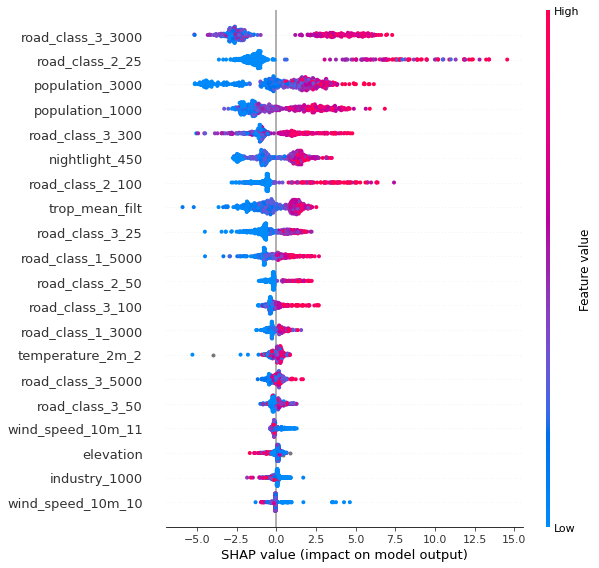
\includegraphics[scale = 0.5]{fig/xgbshap.png}
\caption{Variable impact calculated by SHAP, the XGBoost model. The horizontal location shows whether the effect of that value is associated with a higher or lower prediction.}
\label{xgbshap}
\end{figure}


\section{Discussion}
The advantage of INLA.


\newpage
\bibliographystyle{plain}
\bibliography{references}
\end{document}

Other: the newest boosting technique, Catboost, gives the best cross validation results, with same learning rate as xgboost and number of iterations. But it's not convenient for now to ensemble it as it is not yet in h2o. 

                    Catboost
RMSE          7.0 
RRMSE         0.3 
IQR           6.4 
rIQR          0.3 
MAE           5.0 
rMAE          0.2 
rsq           0.70 
explained\_var 0.70

with spatial cv
                    INLA 
                    
RMSE          10.0900074
RRMSE          0.3023047
IQR           11.6697717
rIQR           0.3894527
MAE            7.4846970
rMAE           0.2242679
rsq            0.3630397
explained\_var  0.4319317
 
 Lasso
RMSE	10.0900074			
RRMSE	0.3023047			
IQR	11.6697717			
rIQR	0.3894527			
MAE	7.4846970			
rMAE	0.2242679			
rsq	0.3630397			
explained\_var	0.4319317	

RF
RMSE	9.6393525			
RRMSE	0.2888581			
IQR	11.6795936			
rIQR	0.3899266			
MAE	7.2699949			
rMAE	0.2178434			
rsq	0.4176984			
explained\_var	0.4752084			
covprob90	0.9063574	

XGB 
RMSE	9.6618743			
RRMSE	0.2895155			
IQR	10.1181299			
rIQR	0.3379141			
MAE	7.0342845			
rMAE	0.2107836			
rsq	0.4140045			
explained\_var	0.4960338

Stacked INLA
RMSE           8.48140767
RRMSE          0.25475534
IQR           10.50499614
rIQR           0.35099809
MAE            6.53715007
rMAE           0.19644237
rsq            0.54917218
explained\_var  0.55811686
cor            0.75390795
covprob95      0.21804124
covprob90      0.17989691
covprob50      0.08092784


If I choose clustered points with high prob (big city?), the result is similar to random sampling, and better accuracy. 

 

If I choose scattered points with high prob (does it mean more rural points?), there is very little randomness. result is also worse. --> the reason for scattered points with high prob. is because they contain more info?
there are a lot more clustered points (as the hist. peak at small prob). so the scattered points will be selected first, that is the reason there is little randomness. 

 
\subsection{Variable importance}
   \begin{table}[!htbp] \centering 
    \caption{Variable importance ranked by XGBoost and Random Forest. The ranking is based on variable importance averaged over 20 times bootstrapping.} 
    \label{vimp} 
  \begin{tabular}{@{\extracolsep{5pt}} ccc} 
  \\[-1.8ex]\hline 
  \hline \\[-1.8ex] 
  rank & XGBoost & Random Rorest \\ 
  \hline \\[-1.8ex] 
  1 & population\_3000 & population\_3000 \\ 
  2 & road\_class\_3\_3000 & road\_class\_2\_100 \\ 
  3 & population\_1000 & road\_class\_3\_3000 \\ 
  4 & nightlight\_450 & population\_1000 \\ 
  5 & road\_class\_2\_100 & nightlight\_450 \\ 
  6 & road\_class\_3\_300 & nightlight\_3150 \\ 
  7 & road\_class\_1\_5000 & population\_5000 \\ 
  8 & nightlight\_3150 & road\_class\_3\_300 \\ 
  9 & road\_class\_3\_100 & nightlight\_900 \\ 
  10 & population\_5000 & road\_class\_3\_5000 \\ 
  11 & trop\_mean\_filt & road\_class\_2\_300 \\ 
  12 & radiation & road\_class\_3\_100 \\ 
  13 & nightlight\_900 & nightlight\_4950 \\ 
  14 & road\_class\_3\_5000 & trop\_mean\_filt \\ 
  15 & road\_class\_1\_100 & road\_class\_1\_5000 \\ 
  16 & nightlight\_4950 & industry\_5000 \\ 
  17 & temperature\_2m\_2 & road\_class\_1\_3000 \\ 
  18 & road\_class\_1\_3000 & temperature\_2m\_2 \\ 
  19 & elevation & road\_class\_2\_500 \\ 
  20 & industry\_5000 & elevation \\ 
 
  \hline \\[-1.8ex] 
  \end{tabular} 
  \end{table} 